%%%%%%%%%%%%%%%%%%%%%%%%%%%%%%%%%%%%%%%%%%%%%%%%%%%%%%%%%%%%%%%%%%%%%%%%%
% This file is part of the LaTeX sources of the OMDoc 1.6 specification
% Copyright (c) 2006 Michael Kohlhase
% This work is licensed by the Creative Commons Share-Alike license
% see http://creativecommons.org/licenses/by-sa/2.5/ for details
% The source original is at https://github.com/KWARC/OMDoc/doc/spec 
%%%%%%%%%%%%%%%%%%%%%%%%%%%%%%%%%%%%%%%%%%%%%%%%%%%%%%%%%%%%%%%%%%%%%%%%%

\begin{omgroup}[id=complex-theories,short=Complex Theories,
                            creators=miko,contributors=frabe]
                           {Complex Theories (Modules   {\CTHmodule{spec}} and {\DGmodule{spec}})}

In {\sref{theories-contexts}} we have presented a notion of theory and inheritance that is
sufficient for simple applications like content dictionaries that informally (though
presumably rigorously) define the static meaning of symbols. Experience in e.g. program
verification has shown that this infrastructure is insufficient for large-scale
developments of formal specifications, where reusability of formal components is the key
to managing complexity. For instance, for a theory of rings we cannot simply inherit the
same theory of monoids as both the additive and multiplicative structure.

In this chapter, we will generalize the {\twintoo{inheritance}{relation}} from
{\sref{theories-contexts}} to that of ``{\twintoo{theory}{inclusion}s}'', also called
``{\twintoo{theory}{morphism}s}'' or ``{\twintoo{theory}{interpretation}s}''
elsewhere~\cite{Farmer93}.  This infrastructure allows to structure a collection of
theories into a complex theory graph that particularly supports modularization and reuse
of parts of specifications and theories. This gives rise to the name ``complex theories''
of the {\omdoc} module.

\begin{presonly}
\begin{myfig}{cpx-thy}{Complex Theories in {\omdoc}}
\begin{scriptsize}
\begin{tabular}{|>{\tt}l|>{\tt}p{1.1truecm}|>{\tt}p{3.3truecm}|c|>{\tt}p{2.9truecm}|}\hline
{\rm Element}& \multicolumn{2}{l|}{Attributes\hspace*{2.25cm}}  & M & Content  \\\hline
             & {\rm Required} & {\rm Optional}                  & D &           \\\hline\hline
 theory      &                & xml:id, class, style            & +  & 
             (\llquote{top-level} | imports | inclusion)*\\\hline
 imports     & from           & xml:id, type, class, style,     
                                conservativity, conservativity-just & + & morphism? \\\hline
 morphism    &                & xml:id, base, class, style, type, hiding, consistency, exhaustivity & -- & 
                                 requation*, measure?, ordering? \\\hline
 inclusion   & via            & xml:id, conservativity, 
                                conservativity-just              & -- & EMPTY \\\hline
 theory-inclusion & from, to
                              & xml:id, class, style,     
                                conservativity, conservativity-just & +  &
                                           (CMP*,FMP*, morphism, obligation*)\\\hline
 axiom-inclusion  & from, to  & xml:id, class, style,     
                                conservativity, conservativity-just & +  &
                                           morphism?, obligation*\\\hline
\end{tabular}
\end{scriptsize}
\end{myfig}
\end{presonly}

\begin{omgroup}[id=morphisms]{Inheritance via Translations}
\begin{module}[id=morphisms]

Literal inheritance of symbols is often insufficient to re-use mathematical structures and
theories efficiently. Consider for instance the situation in the elementary
{\twintoo{algebraic}{hierarchy}}: for a theory of rings, we should be able to inherit the
additive group structure from the theory {\snippet{group}} of groups and the structure of
a multiplicative monoid from the theory {\snippet{monoid}}: A ring is a set $R$ together
with two operations $+$ and $*$, such that $(R,+)$ is a group with unit $0$ and inverse
operation $-$ and $(R^*,*)$ is a monoid with unit $1$ and base set $R^*\deq\setst{r\in
  R}{r\ne 0}$.  Using the literal inheritance regime introduced so far, would lead us into
a duplication of efforts as we have to define theories for semigroups and monoids for the
operations $+$ and $*$ (see {\myfigref{rings-simple}}).
\begin{myfig}{rings-simple}{A Theory of Rings via Simple Inheritance}
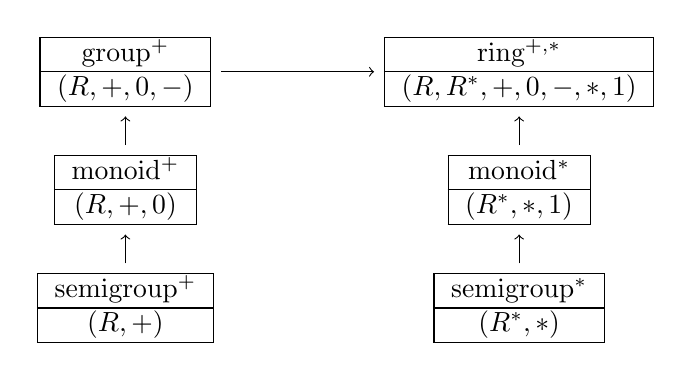
\begin{tikzpicture}
\node (sg) at (1,1)
    {\begin{tabular}{|c|}\hline 
      semigroup$^+$\\\hline
      $(R,+)$\\\hline
    \end{tabular}};
\node (mon) at (1,2.5)
    {\begin{tabular}{|c|}\hline 
      monoid$^+$\\\hline
      $(R,+,0)$\\\hline
    \end{tabular}};
\node (grp) at (1,4)
    {\begin{tabular}{|c|}\hline 
      group$^+$\\\hline
      $(R,+,0,-)$\\\hline
    \end{tabular}};
\node (ring) at (6,4)
    {\begin{tabular}{|c|}\hline 
      ring$^{+,*}$\\\hline
      $(R,R^*,+,0,-,*,1)$\\\hline
    \end{tabular}};
\node (sg1) at (6,1)
    {\begin{tabular}{|c|}\hline 
      semigroup$^*$\\\hline
      $(R^*,*)$\\\hline
    \end{tabular}};
\node (mon1) at (6,2.5)
    {\begin{tabular}{|c|}\hline 
      monoid$^*$\\\hline
      $(R^*,*,1)$\\\hline
    \end{tabular}};

\draw[->](sg)   -- (mon);
\draw[->](sg1)  -- (mon1); 
\draw[->](mon)  -- (grp); 
\draw[->](mon1) -- (ring); 
\draw[->](grp)  -- (ring); 
\end{tikzpicture}
\end{myfig}
  
\begin{omtext}
  This problem\footnote{which seems negligible in this simple example, but in real life,
    each instance of multiple inheritance leads to a {\emph{multiplication}} of all
    dependent theories, which becomes an exponentially redundant management nightmare.}
  can be alleviated by allowing theory inheritance via translations.  Instead of literally
  inheriting the symbols and axioms from the source theory, we involve a symbol mapping
  function (\inlinedef{we call this a {\defin{morphism}}}) in the process. This function
  maps source formulae (i.e. built up exclusively from symbols visible in the source
  theory) into formulae in the target theory by translating the source symbols.
\end{omtext}

\begin{omtext}
{\myfigref{rings-math}} shows a theory graph that defines a theory of rings by importing
the monoid axioms via the morphism $\sigma$. With this translation, we do not have to
duplicate the {\snippet{monoid}} and {\snippet{semigroup}} theories and can even move the
definition of $\cdot^*$ operator into the theory of monoids, where it intuitively
belongs\footnote{On any monoid $M=(S,\circ,e)$, we have the $\cdot^*$ operator, which
  converts a set $S\subseteq M$ in to $S^*\deq\setst{r\in S}{r\ne e}$}.
\end{omtext}

\begin{myfig}{rings-math}{A Theory of Rings via Morphisms}
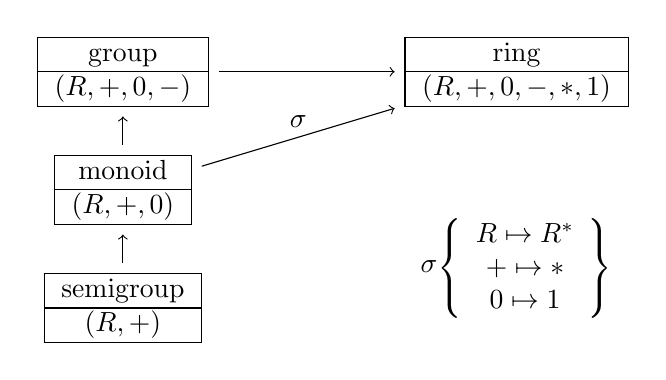
\begin{tikzpicture}
\node (sg) at (1,1)
    {\begin{tabular}{|c|}\hline 
      semigroup\\\hline
      $(R,+)$\\\hline
    \end{tabular}};
\node (mon) at (1,2.5)
    {\begin{tabular}{|c|}\hline 
      monoid\\\hline
      $(R,+,0)$\\\hline
    \end{tabular}};
\node (grp) at (1,4)
    {\begin{tabular}{|c|}\hline 
      group\\\hline
      $(R,+,0,-)$\\\hline
    \end{tabular}};

\node (ring) at (6,4)
    {\begin{tabular}{|c|}\hline 
      ring\\\hline
      $(R,+,0,-,*,1)$\\\hline
    \end{tabular}};
\node (sig) at (6,1.5)
   {$\sigma\deq\scriptscriptstyle\left\{\begin{array}{c}
      R\mapsto R^*\\+\mapsto *\\0\mapsto 1
    \end{array}\right\}$};

\draw[->](sg) -- (mon);
\draw[->](mon) -- (grp);
\draw[->](mon) -- node[above] {$\sigma$} (ring);
\draw[->](grp) -- (ring);
\end{tikzpicture}
\end{myfig}

\begin{omtext}
Formally, we extend the notion of inheritance given in {\sref{theories-contexts}} by allowing a
{\twintoo{target}{theory}} to \inlinedef{import another a {\twintoo{source}{theory}}
  {\defin{via a morphism}}}: Let $\cS$ be a theory with theory-constitutive
elements\footnote{which may in turn be inherited from other theories} $t_1,\ldots,t_n$ and
$\sigma\colon\cS\to\cT$ a morphism, if we declare that $\cT$ imports $\cS$ via $\sigma$,
\inlinedef{then $\cT$ {\defin{inherit}s} the theory-constitutive statements $\sigma(t_i)$
  from $\cS$}. For instance, the theory of rings inherits the {\indextoo{axiom}}
$\allcdot{x}{x+0=x}$ from the theory of monoids as
$\sigma(\allcdot{x}{x+0=x})=\allcdot{x}{x*1=x}$.
\end{omtext}

\begin{definition}[id=morphism.def]
  To specify the formula mapping function, module {\CTHmodule{spec}} extends the
  {\element{imports}} element by allowing it to have a child element {\eldef{morphism}},
  which specifies a formula mapping by a set of recursive equations using the
  {\element{requation}} element described in {\sref{definitions}}. The optional attribute
  {\attribute{type}{morphism}} allows to specify whether the function is really recursive
  (value {\attval{recursive}{type}{morphism}}) or pattern-defined (value
  {\attval{pattern}{type}{morphism}}).
\end{definition}

As in the case of the {\element{definition}} element, termination of the defined function
can be specified using the optional child elements {\element{measure}} and
{\element{ordering}}, or the optional attributes {\attribute{uniqueness}{morphism}} and
{\attribute{existence}{morphism}}, which point to uniqueness and existence
assertions. {\indexalt{Consistency}{consistency}} and {\indextoo{exhaustivity}} of the
recursive equations are specified by the optional attributes
{\attribute{consistency}{morphism}} and {\attribute{exhaustivity}{morphism}}.

{\Mylstref{rings}} gives the {\omdoc} representation of the theory graph in
{\myfigref{rings-math}}, assuming the theories in {\mylstref{def-group}}.

\begin{lstlisting}[label=lst:rings,
  caption={A Theory of Rings by Inheritance Via Renaming},
  index={derive,method,premise}]
<theory xml:id="ring"> 
  <symbol name="times"/><symbol name="one"/> 
  <imports xml:id="add.import" from="#group" type="global"/>
  <imports xml:id="mult.import" from="#monoid" type="global"> 
    <morphism> 
      <requation> 
        <OMS cd="monoid" name="set"/>
        <OMA><OMS cd="monoid" name="setstar"/>
          <OMS cd="semigroup" name="set"/>
        </OMA>
      </requation> 
      <requation> 
        <OMS cd="monoid" name="op"/>
        <OMS cd="ring" name="times"/>
      </requation> 
      <requation>
        <OMS cd="monoid" name="neut"/>
        <OMS cd="ring" name="one"/>
      </requation> 
    </morphism> 
  </imports> 
  <axiom xml:id="ring.distribution"> 
    <CMP><OMS cd="semigroup" name="op"/> distributes over 
      <OMS cd="ring" name="times"/> 
    </CMP> 
  </axiom>
</theory>
\end{lstlisting}

To conserve space and avoid redundancy, {\omdoc} morphisms need only specify the values of
symbols that are translated; all other symbols are inherited literally.  Thus the set of
symbols inherited by an {\element{imports}} element consists of the symbols of the source
theory that are not in the domain of the morphism. In our example, the symbols $R$, $+$,
$0$, $-$, $*$, $1$ are visible in the theory of rings (and any other symbols the theory of
semigroups may have inherited). Note that we do not have a name clash from multiple
inheritance.
  
Finally, it is possible to hide symbols from the source theory by specifying them in the
{\attribute{hiding}{morphism}} attribute. The intended meaning is that the underlying
signature mapping is defined (total) on all symbols in the source theory except on the
hidden ones. This allows to define symbols that are local to a given theory, which helps
achieve data protection. Unfortunately, there is no simple interpretation of hiding in the
general case in terms of formula translations, see~\cite{CoFI:2004:CASL-RM,MAH-06-a} for
details. The definition of hiding used there is more general. The variant used here arises
as the special case where the hiding morphism, which goes against the import direction, is
an inclusion; then the symbols that are not in the image are the hidden ones.  If we
restrict ourselves to hiding defined symbols, then the situation becomes simpler to
understand: A morphism that hides a (defined) symbol $s$ will translate the
theory-constitutive elements of the source theory by expanding definitions. Thus $s$ will
not be present in the target theory, but all the contributions of the theory-constitutive
elements of the source theory will have been inherited. Say, we want to define the concept
of a sorting function, i.e. a function that --- given a list $L$ as input --- returns a
returns a permutation $L'$ of $L$ that is ordered. In the situation depicted in
{\myfigref{rest:actualization}}, we would the concept of an ordering function (a function
that returns a permutation of the input list that is ordered) with the help of predicates
{\snippet{perm}} and {\snippet{ordered}}. Since these are only of interest in the context
of the definition of the latter, they would typically be hidden in order to refrain from
polluting the name space.

As morphisms often contain common prefixes, the {\element{morphism}} element has an
optional {\attribute{base}{morphism}} attribute, which points to a chain of morphisms,
whose {\indextoo{composition}} is taken to be the base of this morphism. The intended
meaning is that the new morphism coincides as a function with the base morphism, wherever
the specified pattern do not match, otherwise their corresponding values take precedence
over those in the {\twintoo{base}{morphism}}.  Concretely, the
{\attribute{base}{morphism}} contains a whitespace-separated list of
{\twintoo{URI}{reference}s} to {\element{theory-inclusion}}, {\element{axiom-inclusion}},
and {\element{imports}} elements. Note that the order of the references matters: they are
ordered in order of the path in the local chain, i.e if we have
{\snippet{base="\#\llquote{ref1}\ldots \#\llquote{refn}"}} there must be theory inclusions
$\sigma_i$ with {\snippet{xml:id="}\llquote{refi}\snippet{"}}, such that the target theory
of $\sigma_{i-1}$ is the source theory of $\sigma_i$, and such that the source theory of
$\sigma_1$ and the target theory of $\sigma_n$ are the same as those of the current theory
inclusion.

Finally, the {\CTHmodule{spec}} module adds two the optional attributes
{\attribute{conservativity}{imports}} and {\attribute{conservativity-just}{imports}} to
the {\element{imports}} element for stating and justifying {\indextoo{conservativity}}
(see the discussion below).
\end{module}
\end{omgroup}

\begin{omgroup}[id=theory-inclusions]{Postulated Theory Inclusions}
\begin{module}[id=theory-morphisms]

We have seen that inheritance via morphisms provides a powerful mechanism for structuring
and re-using theories and contexts. It turns out that the distinguishing feature of theory
morphisms is that all theory-constitutive elements of the source theory are valid in the
target theory (possibly after translation). This can be generalized to obtain even more
structuring relations and thus possibilities for reuse among theories. Before we go into
the {\omdoc} infrastructure, we will briefly introduce the mathematical model (see
e.g.~\cite{Hutter:mocsv00} for details).

\begin{definition}[display=flow,id=theory-inclusion.def]
  A {\twindef{theory}{inclusion}} from a {\twindef{source}{theory}} $\cS$ to a
  {\twindef{target}{theory}} $\cT$ is a mapping $\sigma$ from $\cS$
  objects\footnote{Mathematical objects that can be represented using the only symbols of
    the source theory $\cS$.} to those of $\cT$, such that for every theory-constitutive
  statement $\bS$ of $\cS$, $\sigma(\bS)$ is provable in $\cT$ (we say that $\sigma(\bS)$
  is a {\defin[theorem-of]{$\cT$-theorem}}).
\end{definition}   

In {\omdoc}, we weaken this logical property to a structural one: 
\begin{definition}[id=structurally-included.def,display=flow]
  We say that a theory-constitutive statement $\bS$ in theory $\cS$ is
  {\twindef{structurally}{included}} in theory $\cT$ via $\sigma$, if there is an
  \twintoo{assertional}{element} $\bT$ in $\cT$, such that the content of $\bT$ is
  $\sigma(\bS)$.
\end{definition}
Note that strictly speaking, $\sigma$ is only defined on formulae, so that if a statement
$\bS$ is only given by a {\element{CMP}}, $\sigma(\bS)$ is not defined. In such cases, we
assume $\sigma(\bS)$ to contain a {\element{CMP}} element containing suitably translated
mathematical vernacular.

\begin{definition}[id=structural.theory.inclusion.def]
  In this view, a {\atwindef{structural}{theory}{inclusion}} from $\cS$ to $\cT$ is a
  morphism $\sigma\colon\cS\to\cT$, such that every theory-constitutive element is
  structurally included in $\cT$.
\end{definition}

\begin{omtext}
Note that an {\element{imports}} element in a theory $\cT$ with source theory $\cS$ as
discussed in {\sref{morphisms}} induces a theory inclusion from $\cS$ into
$\cT$\footnote{Note that in contrast to the inheritance relation induced by the
  {\element{imports}} elements the relation induced by general theory inclusions may be
  cyclic. A cycle just means that the theories participating in it are semantically
  equivalent.} (the theory-constitutive statements of $\cS$ are accessible in $\cT$ after
translation and are therefore structurally included trivially).  \inlinedef{We call this
  kind of theory inclusion \atwinalt
  {\defin{definitional}}{definitional}{theory}{inclusion}, since it is a theory inclusion
  by virtue of the definition of the target theory}.  For all other theory inclusions
(\inlinedef{we call them {\atwindef{postulated}{theory}{inclusion}s}}), we have to
establish the theory inclusion property by proving the translations of the
theory-constitutive statements of the source theory (\inlinedef{we call these translated
  formulae {\twindef{proof}{obligation}}}).
\end{omtext}

\begin{omtext}
  The benefit of a theory inclusion is that all {\indextoo{theorem}s},
  {\indextoo{proof}s}, and {\twintoo{proof}{method}s} of the source theory can be used
  (after translation) in the target theory (see {\sref{induced-assertions}}).  Obviously,
  the transfer approach only depends on the theorem inclusion property, and we can extend
  its utility by augmenting the theory graph by more theory morphisms than just the
  definitional ones (see~\cite{FaGu93} for a description of the {\imps} theorem proving
  system that makes heavy use of this idea).  We use the infrastructure presented in this
  chapter to structure a collection of theories as a {\indextoo{graph}} --- \inlinedef{the
    {\twindef{theory}{graph}}} --- where the nodes are theories and the links are theory
  inclusions (definitional and postulated ones).
\end{omtext}

\begin{definition}[display=flow,id=conservative.def]
  We call a theory inclusion $\sigma\colon\cS\to\cT$ {\defin{conservative}}, iff $\bA$ is
  already a $\cS$-theorem for all $\cT$-theorems of the from $\sigma(\bA)$.
\end{definition}
If the morphism $\sigma$ is the identity, then this means the local axioms in $\cT$ only
affect the local symbols of $\cT$, and do not the part inherited from $\cS$. In
particular, conservative extensions of consistent theories cannot be inconsistent. For
instance, if all the local theory-constitutive elements in $\cT$ are symbol declarations
with definitions, then conservativity is guaranteed by the special form of the
definitions. We can specify conservativity of a theory inclusion via the
{\attributeshort{conservativity}}. The values {\attvalshort{conservative}{conservativity}}
and {\attvalshort{conservative}{definitional}} are used for the two cases discussed
above. There is a third value: {\attvalshort{conservative}{conservativity}}, which we will
not explain here, but refer the reader to~\cite{MAH-06-a}.

\begin{definition}[id=theory-inclusion.def]
  {\omdoc} implements the concept of postulated theory inclusions in the
  {\indextoo{top-level}} {\eldef{theory-inclusion}} element. It has the required
  attributes {\attribute{from}{theory-inclusion}} and {\attribute{to}{theory-inclusion}},
  which point to the source- and target theories and contains a {\element{morphism}} child
  element as described above to define the translation function. A subsequent (possibly
  empty) set of {\element{obligation}} elements can be used to mark up proof obligations
  for the theory-constitutive elements of the source theory.
\end{definition}

\begin{definition}[id=obligation.def]
  An {\eldef{obligation}} is an empty element whose {\attribute{assertion}{obligation}}
  attribute points to an {\element{assertion}} element that states that the
  theory-constitutive statement specified by the {\attribute{induced-by}{obligation}}
  (translated by the morphism in the parent {\element{theory-inclusion}}) is provable in
  the target theory.  Note that a {\element{theory-inclusion}} element must contain
  {\element{obligation}} elements for all theory-constitutive elements (inherited or
  local) of the source theory to be correct.
\end{definition}

{\mylstref{theory-inclusion}} shows a theory inclusion from the theory {\snippet{group}}
defined in {\mylstref{def-group}} to itself. The morphism just maps each element of the
base set to its inverse. A good application for this kind of theory morphism is to import
claims for symmetric (e.g. with respect to the function {\snippet{inv}}, which serves as
an involution in {\snippet{group}}) cases via this theory morphism to avoid explicitly
having to prove them (see {\sref{induced-assertions}}).

\begin{lstlisting}[label=lst:theory-inclusion,mathescape,
  caption={A Theory Inclusion for Groups},
  index={theory-inclusion,morphism,requation,assertion}]
<assertion xml:id="conv.assoc">$\allcdot{x,y,z\in{M}}{z\circ(y\circ x)=(z\circ y)\circ x}$</assertion>
<assertion xml:id="conv.closed" theory="semigroup">$\allcdot{x,y\in{M}}{y\circ x\in{M}}$</assertion>
<assertion xml:id="left.unit" theory="monoid">$\allcdot{x\in{M}}{e\circ x= x}$</assertion>
<assertion xml:id="conv.inv" theory="group">$\allcdot{x,y\in{M}}{x\circ x^{-1}=e}$</assertion>
<theory-inclusion xml:id="grp-conv-grp" from="#group" to="#group">
  <morphism><requation>$X\circ Y\leadsto Y\circ X$</requation></morphism>
  <obligation assertion="#conv.closed" induced-by="#closed.ax"/>
  <obligation assertion="#conv.assoc" induced-by="#assoc.ax"/>
  <obligation assertion="#left.unit" induced-by="#unit.ax"/>
  <obligation assertion="#conv.inv" induced-by="#inv.ax"/>
</theory-inclusion>  
\end{lstlisting}
\end{module}
\end{omgroup}

\begin{omgroup}[id=restricting-inference,short=Local/Required Theory Inclusions]{Local- and
  Required Theory Inclusions}
\begin{module}[id=restinf]

In some situations, we need to pose well-definedness conditions on theories, e.g. that a
specification of a program follows a certain security model, or that a parameter theory
used for actualization satisfies the assumptions made in the formal parameter theory; (see
{\extref{primer}{natlist}} for a discussion). If these conditions are not met, the theory
intuitively does not make sense. So rather than simply stating (or importing) these
assumptions as theory-constitutive statements --- which would make the theory
inconsistent, when they are not met --- they can be stated as well-definedness
conditions. Usually, these conditions can be posited as theory inclusions, so checking
these conditions is a purely structural matter, and comes into the realm of {\omdoc}'s
structural methods.

\begin{definition}[id=inclusion.def] 
  {\omdoc} provides the empty {\eldef{inclusion}} element for this purpose. It can occur
  anywhere as a child of a {\element{theory}} element and its {\attribute{via}{inclusion}}
  attribute points to a theory inclusion, which is required to hold in order for the
  parent theory to be well-defined.
\end{definition}  

If we consider for instance the situation in {\myfigref{rest:actualization}}\footnote{This
  example is covered in detail in {\extref{primer}{natlist}}.}.  There we have a theory
{\snippet{OrdList}} of lists that is generic in the elements (which is assumed to be a
totally ordered set, since we want to talk about ordered lists). We want to to instantiate
{\snippet{OrdList}} by applying it to the theory {\snippet{NatOrd}} of natural numbers and
obtain a theory {\snippet{NatOrdList}} of lists of natural numbers by importing the theory
{\snippet{OrdList}} in {\snippet{NatOrdList}}. This only makes sense, if
{\snippet{NatOrd}} is a totally ordered set, so we add an {\element{inclusion}} element in
the statement of theory {\snippet{NatOrdList}} that points to a theory inclusion of
{\snippet{TOSet}} into {\snippet{OrdNat}}, which forces us to verify the axioms of
{\snippet{TOSet}} in {\snippet{OrdNat}}.

\begin{myfig}{rest:actualization}{A Structured Specification of Lists (of
    Natural Numbers)}
  \begin{tikzpicture}\infigures{actualization}\end{tikzpicture}\quad
  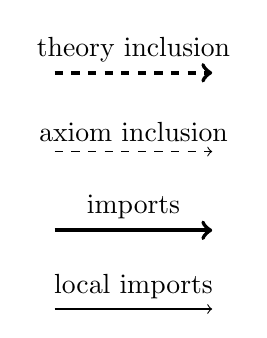
\begin{tikzpicture}
    \draw[->,dashed,line width=1.5pt] (0,3) -- node[above]{theory inclusion} (2,3);
    \draw[->,dashed] (0,2) -- node[above]{axiom inclusion} (2,2);
    \draw[->,line width=1.5pt] (0,1) -- node[above]{imports} (2,1);
    \draw[->] (0,0) -- node[above]{local imports} (2,0);
 \end{tikzpicture}
\end{myfig}

Furthermore note, that the inclusion of {\snippet{OrdList}} into {\snippet{NatOrdList}}
should not include the {\snippet{TOSet}} axioms on orderings, since this would defeat the
purpose of making them a precondition to well-definedness of the theory
{\snippet{NatOrdList}}. Therefore {\omdoc} follows the ``development graph model'' put
forward in~\cite{Hutter:mocsv00} and generalizes the notion of theory inclusions even
further:
\begin{definition}[display=flow,id=local.theory.inclusion]
  A formula mapping between theories $\cS$ and $\cT$ is called a
  {\atwindef{local}{theory}{inclusion}} or {\twindef{axiom}{inclusion}}, if the theory
  inclusion property holds for the local theory-constitutive statements of the source
  theory.
\end{definition}
\begin{omtext}
  To distinguish this from the notion of a proper {\twintoo{theory}{inclusion}} --- where
  the theory inclusion property holds for all theory constitutive statements of $\cS$
  (even the inherited ones) --- \inlinedef{we call the latter one {\defin{global}}}. Of
  course all global theory inclusions are also local ones, so that the new notion is a
  true generalization. Note that the structural inclusions of an
  {\twintoo{axiom}{inclusion}} are not enough to justify translated source theorems in the
  target theory.
\end{omtext}

\begin{omtext}
  To allow for a local variant of inheritance, the {\CTHmodule{spec}} module adds an
  attribute {\attribute{type}{imports}} to the {\element{imports}} element. This can take
  the values {\attval{global}{type}{imports}} (the default) and
  {\attval{local}{type}{imports}}. In the latter case, only the theory-constitutive
  statements that are local to the source theory are imported.
\end{omtext}

\begin{definition}[id=axiom-inclusion.def]
  Furthermore, the {\CTHmodule{spec}} module introduces the {\eldef{axiom-inclusion}}
  element for {\atwintoo{local}{theory}{inclusion}s}. This has the same attributes as
  {\element{theory-inclusion}}: {\attribute{from}{axiom-inclusion}} to specify source
  theory, {\attribute{to}{axiom-inclusion}} for the target theory. It also allows
  {\element{obligation}} elements as children.
\end{definition}
\end{module}
\end{omgroup}


\begin{omgroup}[id=induced-assertions,short=Induced Assertions]{Induced Assertions and
  Expositions}
\begin{module}[id=assertionvia]

The main motivation of theory inclusions is to be able to transport mathematical
statements from the {\twintoo{source}{theory}} to the {\twintoo{target}{theory}}. In
{\omdoc}, this operation can be made explicit by the attributes
{\attributeshort{generated-from}} and {\attributeshort{generated-via}} that the module
{\CTHmodule{spec}} adds to all {\twintoo{mathematical}{statement}s}.  On a statement
$\bT$, the second attribute points to a {\twintoo{theory}{inclusion}} $\sigma$ whose
target is (imported into the) current theory, the first attribute points to a statement
$\bS$ in that theory which is of the same type (i.e. has the same {\omdoc} element name)
as $\bT$.  The content of $\bT$ must be (equivalent to) the content of $\bS$ translated by
the morphism of $\sigma$.
  
  In the context of the theory inclusion in {\mylstref{theory-inclusion}}, we
  might have the following situation:
\begin{lstlisting}[label=lst:assertion-translation,mathescape,
  caption={Translating a Statement via a Theory Inclusion},
  index={translated-from,translated-via}]
<assertion xml:id="foo" type="theorem">$\ldots$</assertion>
<proof xml:id="foo.pf" for="#foo">$\ldots$</proof>
<assertion xml:id="target" induced-by="#foo" induced-via="#grp-conv-grp"> 
  $\ldots$
</assertion>
\end{lstlisting}
Here, the second assertion is induced by the first one via the theory inclusion in
{\mylstref{theory-inclusion}}, the statement of the theorem is about the inverses.  In
particular, the proof of the second theorem comes for free, since it can also be induced
from the proof of the first one.

In particular we see that in {\omdoc} documents, not all statements are automatically
generated by translation e.g. the proof of the second assertion is not explicitly stated.
Mathematical knowledge management systems like knowledge bases might choose to do so, but
at the document level we do not mandate this, as it would lead to an explosion of the
document sizes. Of course we could cache the transformed proof giving it the same ``cache
attribute state''.

Note that not only statements like assertions and proofs can be translated via theory
inclusions, but also whole documents: Say that we have course materials for elementary
algebra introducing monoids and groups via {\twintoo{left}{unit}s} and
{\twintoo{left}{inverse}s}, but want to use examples and exercises from a book that
introduces them using {\twintoo{right}{unit}s} and {\twintoo{right}{inverse}s}. Assuming
that both are formalized in {\omdoc}, we can just establish a theory morphism much like
the one in {\mylstref{theory-inclusion}}. Then we can automatically translate the
exercises and examples via this theory inclusion to our own setting by just applying the
morphism to all formulae in the text\footnote{There may be problems, if mathematical
  statements are verbalized; this can currently not be translated directly, since it would
  involve language processing tools much beyond the content processing tools described in
  this {\report}. For the moment, we assume that the materials are written in a controlled
  subset of mathematical vernacular that avoids these problems.}  and obtain exercises and
examples that mesh well with our introduction. Of course there is also a theory inclusion
in the other direction, which is an inverse, so our colleague can reuse our course
materials in his right-leaning setting.

Another example is the presence of different normalization factors in physics or branch
cuts in elementary complex functions. In both cases there is a plethora of definitions,
which all describe essentially the same objects (see e.g.~\cite{BraCor:raefca02} for an
overview over the branch cut situation). Reading materials that are based on the ``wrong''
definition is a nuisance at best, and can lead to serious errors. Being able to adapt
documents by translating them from the author theory to the user theory by a previously
established theory morphism can alleviate both.

Mathematics and science are full of such situations, where objects can be viewed from
different angles or in different representations. Moreover, no single representation is
``better'' than the other, since different views reveal or highlight different aspects of
the object (see~\cite{KohKoh:esmk05} for a systematic account). Theory inclusions seem
uniquely suited to formalize the structure of different views in mathematics and their
interplay, and the structural markup for theories in {\omdoc} seems an ideal platform for
offering added-value services that feed on these structures without committing to a
particular formalization or foundation of mathematics.
\end{module}
\end{omgroup}

\begin{omgroup}[id=development-graphs,short=Development Graphs]{Development Graphs (Module
  {\DGmodule{spec}})}
\begin{module}[id=dgraph]
  
The {\omdoc} module {\DGmodule{spec}} for {\twintoo{development}{graph}s} complements
module {\CTHmodule{spec}} with high-level justifications for the theory inclusions.
Concretely, the module provides an infrastructure for dealing efficiently with the proof
obligations induced by theory inclusions and forms the basis for a
\twinalt{managementoftheory change}{management}{change}. We anticipate that the elements
introduced in this chapter will largely be hidden from the casual user of mathematical
software systems, but will form the basis for high-level document- and
{\atwintoo{mathematical}{knowledge}{management}} services.

\begin{omgroup}[id=dg-intro,short=Introduction]{Introduction}

As we have seen in the example in {\mylstref{theory-inclusion}}, the burden of specifying
an {\element{obligation}} element for each theory-constitutive element of the source
theory can make the establishment of a theory inclusion quite cumbersome --- theories high
up in inheritance hierarchies can have a lot (often hundreds) of inherited,
theory-constitutive statements.  Even more problematically, such obligations are a source
of redundancy and non-local dependencies, since many of the theory-constitutive elements
are actually inherited from other theories.
  
  Consider for instance the situation in {\myfigref{thi-proof}}, where we are interested
  in the top theory inclusion $\Gamma$. On the basis of theories $\cT_1$ and $\cT_2$,
  theory $\cC_1$ is built up via theories $\cA_1$ and $\cB_1$.  Similarly, theory $\cC_2$
  is built up via $\cA_2$ and $\cB_2$ (in the latter, we have a non-trivial non-trivial
  morphism $\sigma$).  Let us assume for the sake of this argument that for
  $\cX_i\in\{\cA,\cB,\cC\}$ theories $\cX_1$ and $\cX_2$ are so similar that axiom
  inclusions (they are indicated by thin dashed arrows in {\myfigref{thi-proof}} and have
  the formula-mappings $\alpha$, $\beta$, and $\gamma$) are easy to prove\footnote{A
    common source of situations like this is where the $\cX_2$ are variants of the $\cX_1$
    theories. Here we might be interested whether $\cC_2$ still proves the same theories
    (and often also in the converse theory inclusion $\Gamma^{-1}$ that would prove that
    the variants are equivalent).}.

\begin{myfig}{thi-proof}{A Development Graph with Theory Inclusions}
  \begin{scriptsize}
  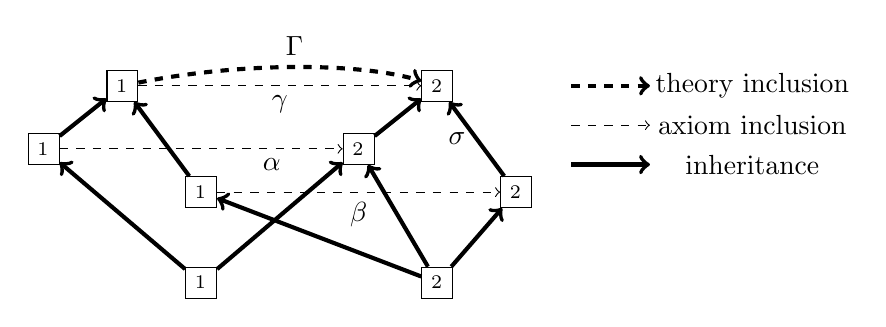
\begin{tikzpicture}
    \begin{scope}
      \tikzstyle{every node}=[draw]
      \node (th1) at (2,-0.5) {$\cT_1$};
      \node (th2) at (5,-0.5) {$\cT_2$};
      \node (a1) at (0,1.2) {$\cA_1$};
      \node (b1) at (2,0.65) {$\cB_1$};
      \node (c1) at (1,2) {$\cC_1$};
      \node (a2) at (4,1.2) {$\cA_2$};
      \node (b2) at (6,0.65) {$\cB_2$};
      \node (c2) at (5,2) {$\cC_2$};
    \end{scope}
    \draw[->,line width=1.5pt](th1) -- (a1);
   \draw[->,line width=1.5pt](th1) -- (a2);
   \draw[->,line width=1.5pt](th2) -- (b1);
   \draw[->,line width=1.5pt](th2) -- (a2);
   \draw[->,line width=1.5pt](th2) -- (b2);
   \draw[->,line width=1.5pt](a1) -- (c1);
   \draw[->,line width=1.5pt](a2) -- (c2);
   \draw[->,line width=1.5pt](b1) -- (c1);
   \draw[->,line width=1.5pt](b2) -- node[left] {$\sigma$} (c2);

   \draw[->,dashed](a1) -- node[below,near end]{$\alpha$} (a2);
   \draw[->,dashed](b1) -- node[below]{$\beta$} (b2);
   \draw[->,dashed](c1) -- node[below]{$\gamma$} (c2);
   \draw[->,dashed,line width=1.5pt] (c1) .. controls (2.5,2.3) and (4,2.3) .. 
       node[above]{$\Gamma$} (c2);
   \draw[->,dashed,line width=1.5pt] (6.7,2) -- (7.7,2);
   \node (ti) at (9,2) {theory inclusion};
   \draw[->,dashed] (6.7,1.5) -- (7.7,1.5);
   \node (ai) at (9,1.5) {axiom inclusion};
   \draw[->,line width=1.5pt] (6.7,1) -- (7.7,1);
   \node (i) at (9,1) {inheritance};
 \end{tikzpicture}
\end{scriptsize}
\end{myfig}

To justify $\Gamma$, we must prove that the
$\Gamma$-translations of all the theory-constitutive statements of $\cC_1$ are provable in
$\cC_2$. So let statement $\bB$ be theory-constitutive for $\cC_1$, say that it is local
in $\cB_1$, then we already know that $\beta(\bB)$ is provable in $\cB_2$ since $\beta$ is
an axiom inclusion. Moreover, we know that $\sigma(\beta(\bB))$ is provable in $\cC_2$,
since $\sigma$ is a (definitional, global) theory inclusion. So, if we have
$\Gamma=\sigma\circ\beta$, then we are done for $\bB$ and in fact for all local statements
of $\cB_1$, since the argument is independent of $\bB$. Thus, we have established the
existence of an axiom inclusion from $\cB_1$ to $\cC_2$ simply by finding suitable
inclusions and checking translation compatibility.

\begin{definition}[id=axiom-inclusion.def]
  We will call a situation, where a theory $\cT$ can be reached by an {\indextoo{axiom
      inclusion}} with a subsequent chain of {\twintoo{theory}{inclusion}s} a
  {\twindef{local}{chain}} (with morphism
  $\tau\colon=\sigma_n\circ\cdots\circ\sigma_1\circ\sigma$), if
  $\cS\stackrel\sigma\longrightarrow\cT_1$ is an {\twintoo{axiom}{inclusion}} or (local
  theory import) and $\cT_i\stackrel{\sigma_i}\longrightarrow\cT_{i+1}$ are
  {\twintoo{theory}{inclusion}s} (or local theory import).
\end{definition}
\begin{center}
  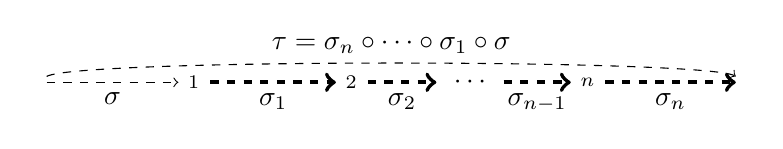
\begin{tikzpicture}
    \node (s) at (0,0) {$\cS$};
    \node (t1) at (2,0) {$\cT_1$};
    \node (t2) at (4,0) {$\cT_2$};
    \node (dots) at (5.5,0) {$\;\cdots\;$};
    \node (tn) at (7,0) {$\cT_n$};
    \node (t) at (9,0) {$\cT$};
    \draw[->,dashed](s) -- node[below]{$\sigma$} (t1);
    \draw[->,line width=1.5pt,dashed](t1) -- node[below]{$\sigma_1$} (t2);
    \draw[->,line width=1.5pt,dashed](t2) -- node[below]{$\sigma_2$} (dots);
    \draw[->,line width=1.5pt,dashed](dots) -- node[below]{$\sigma_{n-1}$} (tn);
    \draw[->,line width=1.5pt,dashed](tn) -- node[below]{$\sigma_n$}(t);
    \draw[->,dashed](s) .. controls (.5,.3) and (8.5,.3) ..
      node[above]{$\tau=\sigma_n\circ\cdots\circ\sigma_1\circ\sigma$} (t);
  \end{tikzpicture}
\end{center}

Note that by an argument like the one for $\bB$ above, a local chain justifies an axiom
inclusion from $\cS$ into $\cT$: all the $\tau$-translations of the local
theory-constitutive statements in $\cS$ are provable in $\cT$.

In our example in {\myfigref{thi-proof}} --- given the obvious compatibility assumptions
on the morphisms which we have not marked in the figure, --- we can justify four new axiom
inclusions from the theories $\cT_1$, $\cT_2$, $\cA_1$, and $\cB_1$ into $\cC_2$ by the
following local chains\footnote{Note for the leftmost two chains use the fact that theory
  inclusions (in our case definitional ones) are also axiom inclusions by
  definition.}.
\begin{center}
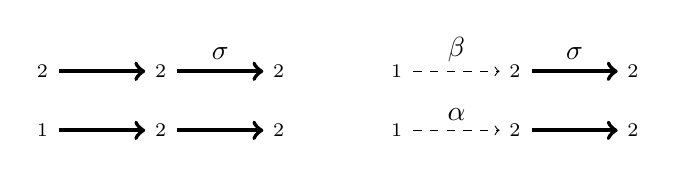
\begin{tikzpicture}
  \node (1) at (0,0) {$\cT_1$};
  \node (2) at (1.5,0) {$\cA_2$};
  \node (3) at (3,0) {$\cC_2$};
  \node (4) at (0,.75) {$\cT_2$};
  \node (5) at (1.5,.75) {$\cB_2$};
  \node (6) at (3,.75) {$\cC_2$};
  \draw[->,line width=1.5pt](1) -- (2);
  \draw[->,line width=1.5pt](2) -- (3);
  \draw[->,line width=1.5pt](4) -- (5);
  \draw[->,line width=1.5pt](5) -- node[above]{$\sigma$} (6);
  \node (7) at (4.5,0) {$\cA_1$};
  \node (8) at (6,0) {$\cA_2$};
  \node (9) at (7.5,0) {$\cC_2$};
  \node (10) at (4.5,.75) {$\cB_1$};
  \node (11) at (6,.75) {$\cB_2$};
  \node (12) at (7.5,.75) {$\cC_2$};
   \draw[->,dashed](7) -- node[above]{$\alpha$} (8);
   \draw[->,line width=1.5pt](8) -- (9);
   \draw[->,dashed](10) -- node[above]{$\beta$} (11);
   \draw[->,line width=1.5pt](11) -- node[above]{$\sigma$} (12);
\end{tikzpicture}
\end{center}

Thus, for each theory $\cX$ that $\cC_1$ inherits from, there is an axiom inclusion into
$\cC_2$. So for any theory-constitutive statement in $\cC_1$ (it must be local in one of
the $\cX$) we know that it is provable in $\cC_2$; in other words $\Gamma$ is a theory
inclusion if it is compatible with the morphisms of these axiom inclusions.  We have
depicted the situation in {\myfigref{thi-proof-decomposition}}.

\begin{myfig}{thi-proof-decomposition}{A Decomposition for the theory inclusion $\Gamma$}
  \begin{scriptsize}
  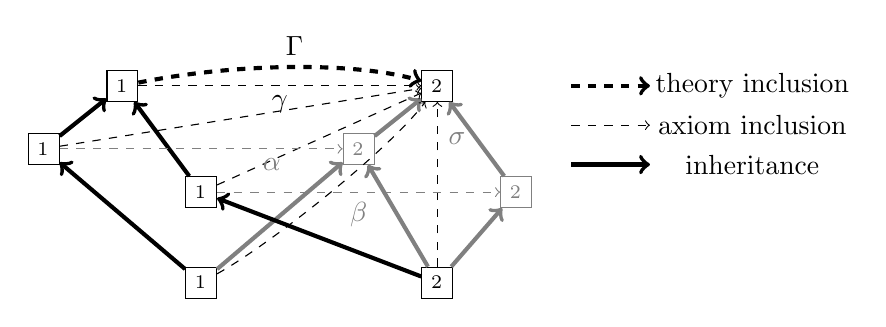
\begin{tikzpicture}
    \begin{scope}
      \tikzstyle{every node}=[draw]
      \node (th1) at (2,-0.5) {$\cT_1$};
      \node (th2) at (5,-0.5) {$\cT_2$};
      \node (a1) at (0,1.2) {$\cA_1$};
      \node (b1) at (2,0.65) {$\cB_1$};
      \node (c1) at (1,2) {$\cC_1$};
      \node[gray] (a2) at (4,1.2) {$\cA_2$};
      \node[gray] (b2) at (6,0.65) {$\cB_2$};
      \node (c2) at (5,2) {$\cC_2$};
    \end{scope}
    \draw[->,line width=1.5pt](th1) -- (a1);
   \draw[->,line width=1.5pt,gray](th1) -- (a2);
   \draw[->,line width=1.5pt](th2) -- (b1);
   \draw[->,line width=1.5pt,gray](th2) -- (a2);
   \draw[->,line width=1.5pt,gray](th2) -- (b2);
   \draw[->,line width=1.5pt](a1) -- (c1);
   \draw[->,line width=1.5pt,gray](a2) -- (c2);
   \draw[->,line width=1.5pt](b1) -- (c1);
   \draw[->,line width=1.5pt,gray](b2) -- node[left] {$\sigma$} (c2);

   \draw[->,dashed](th2) -- (c2);
   \draw[->,dashed](th1) .. controls (2.9,0) and (4.4,1.2) .. (c2);
   \draw[->,dashed](a1) -- (c2);
   \draw[->,dashed](b1) -- (c2);

   \draw[->,dashed,gray](a1) -- node[below,near end]{$\alpha$} (a2);
   \draw[->,dashed,gray](b1) -- node[below]{$\beta$} (b2);
   \draw[->,dashed](c1) -- node[below]{$\gamma$} (c2);
   \draw[->,dashed,line width=1.5pt] (c1) .. controls (2.5,2.3) and (4,2.3) .. 
       node[above]{$\Gamma$} (c2);
   \draw[->,dashed,line width=1.5pt] (6.7,2) -- (7.7,2);
   \node (ti) at (9,2) {theory inclusion};
   \draw[->,dashed] (6.7,1.5) -- (7.7,1.5);
   \node (ai) at (9,1.5) {axiom inclusion};
   \draw[->,line width=1.5pt] (6.7,1) -- (7.7,1);
   \node (i) at (9,1) {inheritance};
 \end{tikzpicture}
\end{scriptsize}
\end{myfig}

\begin{omtext}
We call a situation where we have a formula mapping
$\cS\stackrel\sigma\longrightarrow\cT$, and an axiom inclusion
$\cX\stackrel{\sigma_\cX}\longrightarrow\cT$ for every theory $\cX$ that $\cS$ inherits
from a \inlinedef{{\defin{decomposition}} for $\sigma$, if the $\sigma_\cX$ and $\sigma$
  are compatible}. As we have seen in the example above, a decomposition for $\sigma$ can
be used to justify that $\sigma$ a theory inclusion: all theory-constitutive elements in
$\cS$ are local in itself or one of the theories $\cX$ it inherits from. So if we have
axiom inclusions from all of these to $\cT$, then all obligations induced by them are
justified and $\sigma$ is indeed a theory inclusion.
\end{omtext}
\end{omgroup}

\begin{omgroup}[id=dg-omdoc,short=OMDoc Development Graphs]{An OMDoc Infrastructure for
  Development Graphs (Module {\DGmodule{spec}})}
  
\begin{definition}[id=decomposition.def]
  The {\DGmodule{spec}} module provides the {\eldef{decomposition}} element to model
  justification by decomposition situations.  This empty element can occur at
  {\indextoo{top-level}} or inside a {\element{theory-inclusion}} element.
 
  The {\element{decomposition}} element can occur as a child to a
  {\element{theory-inclusion}} element and carries the required attribute
  {\attribute{links}{decomposition}} that contains a whitespace-separated list of
  {\twintoo{URI}{reference}s} to the {\snippet{axiom-}} and {\element{theory-inclusion}}
  elements that make up the decomposition situation justifying the parent
  {\element{theory-inclusion}} element. Note that the order of references in
  {\attribute{links}{decomposition}} is irrelevant. If the {\element{decomposition}}
  appears on top-level, then the optional {\attribute{for}{decomposition}} attribute must
  be used to point to the {\element{theory-inclusion}} it justifies. In this situation the
  {\element{decomposition}} element behaves towards a {\element{theory-inclusion}} much
  like a {\element{proof}} for an {\element{assertion}}.
\end{definition}

\begin{presonly}
\begin{myfig}{dg-thy}{Development Graphs in {\omdoc}}
\begin{scriptsize}
\begin{tabular}{|>{\tt}l|>{\tt}p{1.3truecm}|>{\tt}p{1.6truecm}|c|>{\tt}p{4.1truecm}|}\hline
{\rm Element}& \multicolumn{2}{l|}{Attributes} & M & Content  \\\hline
             & {\rm Required} & {\rm Optional} & D &           \\\hline\hline
 decomposition  & links       &                            & -- & EMPTY\\\hline
 path-just   & local, globals & for                        & -- & EMPTY\\\hline
 theory-inclusion & from, to, by  
                              & xml:id, class, style               & +  
                                          & (CMP*,FMP*, morphism, 
                                             (decomposition* | obligation*))\\\hline
 axiom-inclusion  & from, to  & xml:id, class, style           & +  
                                          & morphism?, (path-just* | obligation*)\\\hline
\end{tabular}
\end{scriptsize}
\end{myfig}
\end{presonly}

Furthermore module {\DGmodule{spec}} provides {\element{path-just}} elements as children
to the {\element{axiom-inclusion}} elements to justify that this relation holds, much like
a {\element{proof}} element provides a justification for an {\element{assertion}} element
for some property of mathematical objects.

\begin{definition}[id=path-just.def]
  A {\eldef{path-just}} element justifies an {\element{axiom-inclusion}} by reference to
  other {\element{axiom-inclusion}} or {\element{theory-inclusion}}
  elements. \twindefalt{Local chains}{local}{chain} are encoded in the empty
  {\element{path-just}} element via the required attributes {\attribute{local}{path-just}}
  (for the first {\element{axiom-inclusion}}) and the attribute
  {\attribute{globals}{path-just}} attribute, which contains a whitespace-separated list
  of {\twintoo{URI}{reference}s} to {\element{theory-inclusion}s}. Note that the order of
  the references in the {\attribute{globals}{axiom-inclusion}} matters: they are ordered
  in order of the path in the local chain, i.e if we have {\snippet{globals="\ldots{}
      \#ref1 \#ref2 \ldots"}} there must be theory inclusions $\sigma_i$ with
  {\snippet{xml:id="ref$i$"}}, such that the target theory of $\sigma_1$ is the source
  theory of $\sigma_2$.
\end{definition}

Like the {\element{decomposition}} element, {\element{path-just}} can appear at top-level,
if it specifies the {\element{axiom-inclusion}} it justifies in the (otherwise optional)
{\attribute{for}{path-just}} attribute.

Let us now fortify our intuition by casting the situation in {\mylstlref{thi}{thi-proof}}
in {\omdoc} syntax. Another --- more mathematical --- example is carried out in detail in
{\extref{primer}{dg-elal}}.

\begin{lstlisting}[label=lst:thi,mathescape,
                   index={theory,imports,axiom},
                   caption={The {\omdoc} representation of the theories
                   in {\myfigref{thi-proof}}.}]
<theory xml:id="t1">$\ldots$</theory>              <theory xml:id="t2">$\ldots$</theory> 

<theory xml:id="a1">                          <theory xml:id="b1">
  <imports xml:id="ima1" from="#t1"/>           <imports xml:id="imb1" from="#t2"/>
  <axiom xml:id="axa11">$\ldots$</axiom>                 <axiom xml:id="axb11">$\ldots$</axiom>
  <axiom xml:id="axa12">$\ldots$</axiom>               </theory>
</theory>

<theory xml:id="a2">                          <theory xml:id="b2">
  <imports xml:id="im1a2" from="#t1"/>           <imports xml:id="imb2" from="#t2"/>
  <imports xml:id="im2a2" from="#t2"/> 
  <axiom xml:id="axa21">$\ldots$</axiom>                   <axiom xml:id="axb21">$\ldots$</axiom>
</theory>                                     </theory>

<theory xml:id="c1">                          <theory xml:id="c2">
  <imports xml:id="im1c1" from="#a1"/>          <imports xml:id="im1c2" from="#a2"/>
  <imports xml:id="im2c1" from="#b1"/>          <imports xml:id="im2c2" from="#b2"/>
  <axiom xml:id="axc11">$\ldots$</axiom>                  <axiom xml:id="axc21">$\ldots$</axiom>
</theory>                                     </theory>
\end{lstlisting}
Here we set up the theory structure with the theory inclusions given by the
{\element{imports}} elements (without morphism to simplify the presentation). Note
that these have {\attribute[ns-attr=xml]{id}{imports}} attributes, since we need them to
construct axiom- and theory inclusions later. We have also added axioms to induce
proof obligations in the axiom inclusions:
\begin{lstlisting}[label=lst:thi-inclusions,
                   index={obligation,axiom-inclusion},
                   caption={The {\omdoc} Representation of the Inclusions
                   in {\myfigref{thi-proof}}.}]
<axiom-inclusion xml:id="aia" from="#a1" to="#a2">
  <obligation induced-by="#axa11" assertion="#th-axa11"/>
  <obligation induced-by="#axa12" assertion="#th-axa12"/>
</axiom-inclusion>

<axiom-inclusion xml:id="bib" from="#b1" to="#b2"> 
  <obligation induced-by="#axb11" assertion="#th-axb1"/>
</axiom-inclusion>

<axiom-inclusion xml:id="cic" from="#c1" to="#c2">
  <obligation induced-by="#axc11" assertion="#th-axc1"/>
</axiom-inclusion>
\end{lstlisting}
We leave out the actual assertions that justify the {\element{obligation}s} to conserve
space. From the axiom inclusions, we can now build four more via path justifications:

\begin{lstlisting}[label=lst:thi-induced-inclusions,index={path-just,axiom-inclusion},
                   caption={The Induced Axiom Inclusions in {\myfigref{thi-proof}}.}]
<axiom-inclusion xml:id="t1ic" from="#t1" to="#c2">
 <path-just local="#im1a2" globals="#im1c2"/>
</axiom-inclusion>

<axiom-inclusion xml:id="t2ic" from="#t2" to="#c2">
 <path-just local="#imb2" globals="#im2c2"/>
</axiom-inclusion>

<axiom-inclusion xml:id="aic" from="#a1" to="#c2">
 <path-just local="#aia" globals="#im1c2"/>
</axiom-inclusion>

<axiom-inclusion xml:id="bic" from="#b1" to="#c2">
 <path-just local="#bib" globals="#im2c2"/>
</axiom-inclusion>
\end{lstlisting}
Note that we could also have justified the axiom inclusion {\snippet{t2ic}} with
two local paths: via the theory $\cA_2$ and via $\cB_2$ (assuming the translations
work out).  These alternative justifications make the development graph more
robust against change; if one fails, the axiom inclusion still remains justified.
Finally, we can assemble all of this information into a decomposition that
justifies the theory inclusion $\Gamma$:
\begin{lstlisting}[label=lst:thi-proof,index={theory-inclusion,decomposition}
                   caption={Justifying {\element{theory-inclusion}s} via {\element{decompositions}}}]
<theory-inclusion xml:id="tcic" from="#c1" to="#c2">
  <decomposition links="#t1ic #t2ic #aic #bic #cic"/>
</theory-inclusion>
\end{lstlisting}
\end{omgroup}
\end{module}
\end{omgroup}
\end{omgroup}
%%% Local Variables: 
%%% mode: latex
%%% TeX-master: "main"
%%% End: 

% LocalWords:  cpx def requation lst setstar cd mathescape ti thi cic bic aic
% LocalWords:  aia im axa xunit linewidth arcangle ai ima imb axb axc param ord
% LocalWords:  elem toset nat elt nats incl morph natlist dec adt  sg dg truecm
% LocalWords:  mon grp mult tn  TOSet NatOrd sortdef TOset CMP FMP pspic TOSet
% LocalWords:  pt linestyle omdoc elal dgraph conv xref yunit ref ic tcic ns th
% LocalWords:  cpx def requation lst setstar cd mathescape ti thi cic bic aic
% LocalWords:  aia im axa xunit linewidth arcangle ai ima imb axb axc param ord
% LocalWords:  elem toset nat elt nats incl morph natlist dec adt  sg ref conv
% LocalWords:  mon grp mult tn  TOSet NatOrd sortdef TOset OrdList OrdNat TOSet
% LocalWords:  NatOrdList pf attr sig OMA globals refi inv TOSet TOSet
% LocalWords:  TOSet TOSet TOSet TOSet TOSet TOSet TOSet TOSet TOSet TOSet
